\newchap{Linguistic Background}
\label{chap:ling-background}

\review{Add quick intro into corpus linguistics, quantitative analysis, this is essentially what is done with the corpus. \citep{McEnery&Hardie.2011}}

\review{Introduction to comparative linguistics at some place. \citep{Hock&Joseph.2019}} 


Elaborated writing systems like we are used to nowadays came only much later compared to language in general. Can they capture language as such well enough? Computational linguistics deals mostly with written languages, but what does traditional linguistics say about the relation of written and spoken language? Whenever we study language we look at samples of that language. It is simply impossible to study an \textit{entire} language as we would need all texts that were ever produced in that language. Consequently, we need to ask ourselves how much and what material of a language is enough to study it properly \citep{baird_evans_greenhill_2021}. Both written and spoken language are representations of a language. As we will see later in this chapter, mapping a spoken language to its written representation is far from easy and never perfect. \citet{baird_evans_greenhill_2021} focus on answering the question how much phonetic data is needed to represent a language well. We know that each language has specific sounds, its phoneme inventory, that are frequently used. The question is now how much data is needed to cover this entire phoneme inventory of a language. In order to answer that question \citet{baird_evans_greenhill_2021} study \ac{nws} corpus. 

Due to recent technological advancement it has become possible to store large digital collections of speech recordings and their aligned transcriptions. These possibilities gave rise to a wider acknowledgement of corpus phonetics. Corpus phonetics deals with an abundance of linguistic variation. In addition to language, style or vocabulary variation, there are differences in dialect and idiolect, physiological state of the speakers and their attitude \citep{Liberman.2019, Chodroff.19.07.2019}. Many methods and tools used in corpus phonetics are based on \ac{asr} algorithms or simple programming \citep{Chodroff.19.07.2019}.

A way to analyse or use phonetic corpora is to use phonetic features to represent each phoneme. These features are a list of properties that are overlapping with the phonetic description of each phoneme. It is a minimal list that can be used to describe unique phones. In order to do that, it is necessary to understand the basics of written and spoken language. Which is what I will do in this chapter. It covers the basics of phonetics and phonology, writing systems and the relatively new field of corpus phonetics. I will also present the datasets I will be using in this thesis at the end of the chapter. 


There are systems that can produce speech directly from orthography and question the necessity of phonetic transcriptions. When only  little data is available, the training data might not be enough to train a orthography-to-phoneme system, making phonetic transcriptions necessary. Another reason for creating phonetic transcriptions is that it usage is not limited to speech applications \citep{mortensen-etal-2018-epitran}. They might also be used to compare languages on speech basis. In order to do that, there needs to be a lot of knowledge about how language works. Comparing languages and studying their similarities and differences is part of a well-established branch of traditional linguistics called comparative linguistics. The analysis of large amounts of text in any language is commonly referred to as corpus linguistics. Corpus linguistics allows for both qualitative and quantitative analysis of text. Although text can refer to written or spoken language, most corpora contain written text \citep{McEnery&Hardie.2011}. Multilingual corpora can be used to compare languages. If all of these different approaches are combined, we end up by what we could call comparative corpus phonetics. 


\section{Phonemes and syllables}
\label{phonology}
Given that phonetics and phonology is a sub-area of traditional linguistics and often only touched on superficially in computational linguistics, I will summarise the most important assumptions and terms concerning said field. A very important terminological distinction is between phonetics and phonology. While phonetics refers to the study of actual sounds, phonology refers to the study of sound \textit{systems}. In phonetics, it is not so much important what the different sounds mean, but how they are produced and perceived and what different sounds a human being can produce and perceive at all. When it comes to human communication using spoken language, many of these sounds are not actually used to produce distinguishable meaning. This is why on the other hand, phonology is important to describe the set of distinguishable sounds that make up a language. For example: the letter /r/ in English can be pronounced in many different ways in a specific word like `request'. I can roll the /r/ like it is common in Spanish or I can pronounce it like an /r/ in German. None of those pronunciations produces a change in meaning. Others might say I have an accent or I speak a dialect but usually people will understand. This means that there exist many different \textit{phonetic} sounds but only one \textit{phonological} or \textit{phonemic}. Physically, there are many sounds I can produce that map to the /r/, but none of them changes the meaning (at least no in English). Those sounds are referred to as phone and phoneme respectively. While there are infinitely many phones, there are only finitely many phonemes in a language. Also, in one language there is typically a set of phones that is used by the majority of speakers of this language that can replace phonemes and does not change the meaning. Sounds that can replace another sound without changing the original meaning are referred to as `allophones'. Each language has therefore a set of phonemes, a phoneme inventory, and a set of allophones. How phonemes and allophones are used depends a lot on the dialect and idiosyncratic language use.  

Not all different possible sounds are actually considered qualitatively `good' sounds of a language. Usually there is a subset of all possible phones that is accepted as `good quality sounds' within all different dialects of a language \citep{Intro.2007}. An obvious example being loudness: Although very silent speech produces correct phones, these are not `good quality' as they simply cannot be understood. Or speaking in English with hardly any mouth and tongue movement. Although this produces understandable sound, it is not generally considered good speech. 

It is important to note at this point that the terms phonetic and phonemic respectively phone and phoneme are sometimes used interchangeably. Their linguistic definition as given above is clear while the definition on the computational side is often less strict. Strictly speaking phonemic transcriptions are not allowed to contain allophones but should write the respective phoneme of that language. This will not always be the case when it comes to data used in language technology \citep{Lee&Ashby.2020}. 

\subparagraph{Vowels and consonants} Each phone can be described based on different categories. A well-known distinction is that between vowels and consonants. Both of these are again categorized differently. The schema for vowels and consonants is inspired by the human vocal cavity. The terms to describe vowels sounds are based on the position of the tongue in the mouth and if the lips are rounded or not. Using those two categories enables us to distinguish every possible vowel. A vowel can then be described as close-back unrounded (which would be [\ipa{W}]) or open-front rounded ([\ipa{\OE}]). Figure \ref{fig:ipa_chart} shows the vowel chart how it is usually represented in the \ac{ipalpha}. More on this special alphabet and writing systems in general follows in section \ref{sec:ipa}. Consonants are defined by the place and the manner of their production. The place, again, refers to the position of the tongue in the mouth and the overall form of the vocal tract. The vocal tract is used to block the air and make it flow in a specific way. The manner, on the other hand, describes the way the air is lead through the mouth or how it is blocked to produce a sound \citep{phonetics-video}. For dental sounds, the tip of the tongue is moved to the upper middle teeth. For palatal sounds, the body of the tongue is pressed against the hard palate in the back of the mouth cavity. These are examples for places of articulation. Examples for the manner are plosive or trill. A trill makes the tongue move in a vibrating way which consequently makes the air vibrate. A plosive first completely blocks the air and then pushes the air out of the mouth in a fast manner, a bit like an explosion, therefore the name. Both vowel and consonant categorization is rather intuitive and pictorial. The complete consonant chart is depicted in figure \ref{fig:ipa_chart} as well. While the exact description of each phone is not always very important when dealing with computational models for phonetic transcriptions. The key point is that that we can describe sounds uniquely using different features. 

\subparagraph{Syllables} Phonemes, or letters, can be grouped into larger units called \textit{syllables}. Syllables can be an entire word or a part of a word. English syllables typically consist of a group of consonants followed by a group of vowels or a diphthong followed by a group of consonants again. These parts are called \textit{onset}, \textit{nuleus} and \textit{coda} respectively.  For every syllable in every language it is true that the nucleus cannot be empty. The onset and the coda can be empty. Other than that, syllables are organized very differently in different languages \citep{Intro.2007}. For computational analysis it is important that syllables are a way of segmenting written or spoken language. They are larger than individual letters or phonemes but often still smaller than individual morphemes. 

\subparagraph{Diphthongs}
A diphthong is a sequence of vowels that is considered as just one phoneme if is is within one syllable. If a syllable ends with a vowel and the next one starts with a vowel, this vowel sequence is not called a diphthong. An example is the German word `Chaos'. The two vowels in the middle are not a diphthong as there is a syllable boundary right in their middle: `Cha-os'. A word like `aus' contains a diphthong as it exists of only one syllable \citep{Intro.2007}. 

\subparagraph{Suprasegmentals} Apart from individual sounds, there are features of spoken language like stress or intonation. Those are referred to as suprasegmentals. they are often related to syllables. For example, we can put stress on a different syllable or raise the pitch. Semantically, some suprasegmentals in some languages distinguish meanings, some do not. A special case are tones. Tones are a special way of intonation. In some languages like Chinese or many African languages tones are used to distinguish meaning while in most European languages, the concept of tones does not exist \citep{Intro.2007}.


\section{Mappings of written and spoken language}
\label{writing-sys}
Unlike spoken language that was a part of human interaction all the time, writing systems only developed over time. There are different writing systems that developed in different places at different times. The structure of the spoken language, the cultural context or the tools that were at hand to write are a few of many factors that influenced the emergence of a specific writing system. In general, we can think of writing systems as mappings from spoken language to written language. The systems used to represent sounds in different languages do not uniquely map a letter to one specific phoneme. Most of the time, there is a standard pronunciation of each letter that is trained by reciting the alphabet. However, in reciting the alphabet there is a vowel added to the consonants in order to pronounce them more easily. This means that reciting the alphabet is somewhat artificial when compared to what sound is actually produced in natural spoken language. These explanations make clear that the mapping of written text to spoken text in various languages is complex. When taking a step back, we can see that a single grapheme can represent either a phoneme, a syllables or words. The history and development of writing systems is an entire independent study area. For this thesis it is mostly important to be aware of the independently developing systems. Not all scripts can be treated the same and this most certainly has implications on models to create phonetic transcriptions. Each major mapping will be presented below \citep{writing-systems}.

\begin{description}
\item[\textsc{Alphabet}] When a grapheme maps to a phoneme, we call this an alphabet. In German, for example, the writing system consists of the Latin alphabet. The Latin alphabet is used for many different languages in western Europe and those languages that were influence by colonisation. There are other alphabets like the Cyrillic or the Greek alphabet. Having an alphabet does not mean that each grapheme, or letter in this case, maps to exactly one phoneme. In fact, one grapheme can have many different realizations as example \ref{ex:latin-alpha} shows.
\begin{covsubexamples}[preamble={The examples show the different realizations of the English grapheme sequence `ough' \citep{phonetics-video}}]
\label{ex:latin-alpha}
\item tough \>\> [\textipa{t\textturnv f}]
\item cough \>\> [\textipa{k\textturnscripta f}]
\item though \>\> [\textipa{\dh\textschwa\textupsilon}]
\item through \>\> [\textipa{\texttheta ru:}]
\item bough \>\>  [\textipa{baU}] %baʊ
\item brought \>\> [\textipa{brO:t}] %brɔːt
\end{covsubexamples}

The above examples show that it is not possible to have a one-to-one mapping from one grapheme or a sequence of graphemes to one phoneme or a sequence of phonemes with in the English language. Let alone within all languages that use the Latin alphabet. In addition, alphabets typically have diacritic marks that can be used to extend the main letters. Just as with single graphemes, also diacritic marks cannot simply be mapped to a phoneme.

\item[\textsc{Abjad}] A special variant of an alphabet-language is abjad. Abjad represents only consonants and no vowels. This means that vowels need to be added while reading. Again, this means that there is a lot of ambiguity as it is not always clear which vowel should be added if there is no context. Semitic languages like Hebrew or Arabic make use of abjad.

\begin{covsubexamples}[preamble={Hebrew examples that are first mapped to Latin alphabet then to the Latin alphabet including vowels.}]
\label{ex:abjad}
\item \textcjheb{Ml.sb} \>\> bzlm \>\> bzelem
\item \textcjheb{Ml.sb} \>\> bzlm \>\> bzalam
\end{covsubexamples}

Example \ref{ex:abjad} shows that each grapheme maps to a consonant but it can be completed with different vowels. the words presented above do not have the same meaning depending on the vowels added. 

\item[\textsc{Syllabary}] In syllabaries, a grapheme represents a syllable instead of a single sound. Examples are the Japanese Hiragana and Katakana. Both of these examples do not have any internal ambiguities in their pronunciation as one grapheme maps to exactly one phoneme. However, in the case of Japanese, in addition to the syllabaries they use a logographic system as well which is ambiguous.  

\item[\textsc{Logographic systems}] Logographic systems represent entire words or morphemes as graphemes. Chinese is an example for a logographic system. We cannot break down Chinese signs into single morphemes or letters. One sign is typically pronounced in the same way regardless of the context of the sign. Logographic systems are less ambiguous than alphabets for example. 
\end{description}

What all of these mappings have in common is that they are no reliable source of pronunciation as the examples above show \citep{Intro.2007}. Many of the pronunciation rules of a language are based on convention. Speakers of a language just \textit{know} how to pronounce a word. Still, there can arise heated debates about the correct pronunciation of certain words. Just think of Swiss German dialects. Apart from these conventions, spoken and written languages change differently over time. Spoken languages are typically more flexible and ready to change while their written representation often stays the same \citep{unicode-lingu}. This can lead to official governmental interventions like the German orthography reform of 1996 that intended to adapt the German spelling to represent the German pronunciation more adequately. Also, major inventions like printing machines gave rise to standardization of writing systems as reading and writing became more common \citep{writing-systems}.

\section{The International Phonetic Alphabet (IPA)}
\label{sec:ipa}
An exception to the above explained characteristics of an alphabet are phonetic alphabets like the \ac{ipalpha} where each grapheme is intended to represent exactly one phone  \citep{writing-systems, Intro.2007}. As usual, reality is more complex than what we wish it to be. Even with the \ac{ipalpha} there are inconsistencies. Figure \ref{fig:ipa_chart} shows the full \ac{ipalpha} chart including all characters that the \ac{ipa} decided to use. Although the \ac{ipalpha} seems very complete there are still sometimes sounds that cannot be represented using the \ac{ipalpha}. This becomes clear when, for example, looking at the vowel chart (see figure \ref{fig:ipa_chart}). The tongue does not `click into place' for the vowels on the chart. Vowel characterisation happens on a continuum. This means that it is always possible to characterize a vowel as in between two vowels on the chart. The \ac{ipalpha} is not the only transcription convention but by far the most common (at least in this present research setting). 

Apart from different character sets that can be used to represent sounds, there are different levels of detail. Not all transcriptions represent the phonetics in equal detail. Generally, there is the distinction of broad and narrow transcription. These two go back to the linguistic distinction of phone and phoneme. Broad refers to a phonemic description. Following the linguistic definition in chapter \ref{chap:ling-background}, this means that the transcription does not transcribe speaker specific pronunciations or dialectal variations. This kind of transcription is therefore less complex and usually easier to create and understand. Narrow transcriptions are phonetic. They present every speaker individual or dialectal sounds as exactly as possible. Although the spoken text in narrow and broad transcription sounds only minimally different, the two texts can diverge greatly. It is important to treat broad and narrow transcriptions as two different kinds of transcriptions. 

\begin{covexamples}
\item \label{exBro} \textipa{p\textsci\textprimstress kU k9\textprimstress\textrtailz 9f}
\item \label{exNar}\textipa{p\textsci\textprimstress k\super hU k\super h9\textprimstress\textrtailz 9f}
\end{covexamples}

Example \ref{exNar} is a narrow (phonetic) transcription of the beginning of the Mapudungun version of the short story \textit{The North Wind and the Sun}. The same text is transcribed broadly (phonemic) in example \ref{exBro}. As becomes clear in this example, the narrow transcriptions is longer as it contains more different characters. In this case it is only the superscript h that is different. The problem, with especially the narrow transcriptions, is that the transcriber still needs to define what narrow means in a specific case. One could argue that there are as many narrow transcriptions of a language as there are speakers of that language. This becomes tricky when given a task to automatically transcribe text, the training data might employ one definition of narrow, while there are texts in the test set that might follow another definition. This is mostly important when talking about data preprocessing and cleaning.
  
\section{The 100 language corpus}
\label{corpus}
As mentioned in the introduction, the basis of the data used in this thesis is a corpus provided by the SPUR lab at the \ac{uzh}. The corpus contains 100 languages which are proposed by \citet{Comrie&Dryer.2013}. This is an online book that contains different chapters each of which shows a different linguistic feature including a map which shows the distribution of that feature over the world's languages. While the number of languages presented on the individual maps depends on the amount of research done in a specific area, the sum of all maps gives quite an impressive overview on the structure of nearly half of the world's languages. Out of the 2676 languages a sample of 100 languages was chosen. This sample does not contain too many languages from one area, neither does it contain too many languages from one family. Those are the 100 languages that are in the corpus. Not considering the aforementioned criteria of maximizing genealogical and areal diversity can lead to misleading results in multilingual analysis. Figure \ref{fig:100lc} shows the distribution of the corpus on a world map. The different icons show the genus of the languages which is a classification of languages defined by the \ac{wals} team that maintains the language description collection. The interactive map can be viewed online \citep{100LC.21.07.2021}. Table \ref{tab:100LC} in the appendix A shows all languages that are in the 100 language corpus. None of the text samples are provided by \ac{wals}. The entire corpus is provided by the SPUR team that collected the corpus over the last few years and is continuously working on and with it.

\fig{images/100sample.png}{fig:100lc}{WALS - Map that shows the 100 Languages}{\textwidth}{100 Language Map}

\begin{figure}[h]
\vspace*{-1.5cm}
    \begin{center}
    \hspace*{-2cm}
      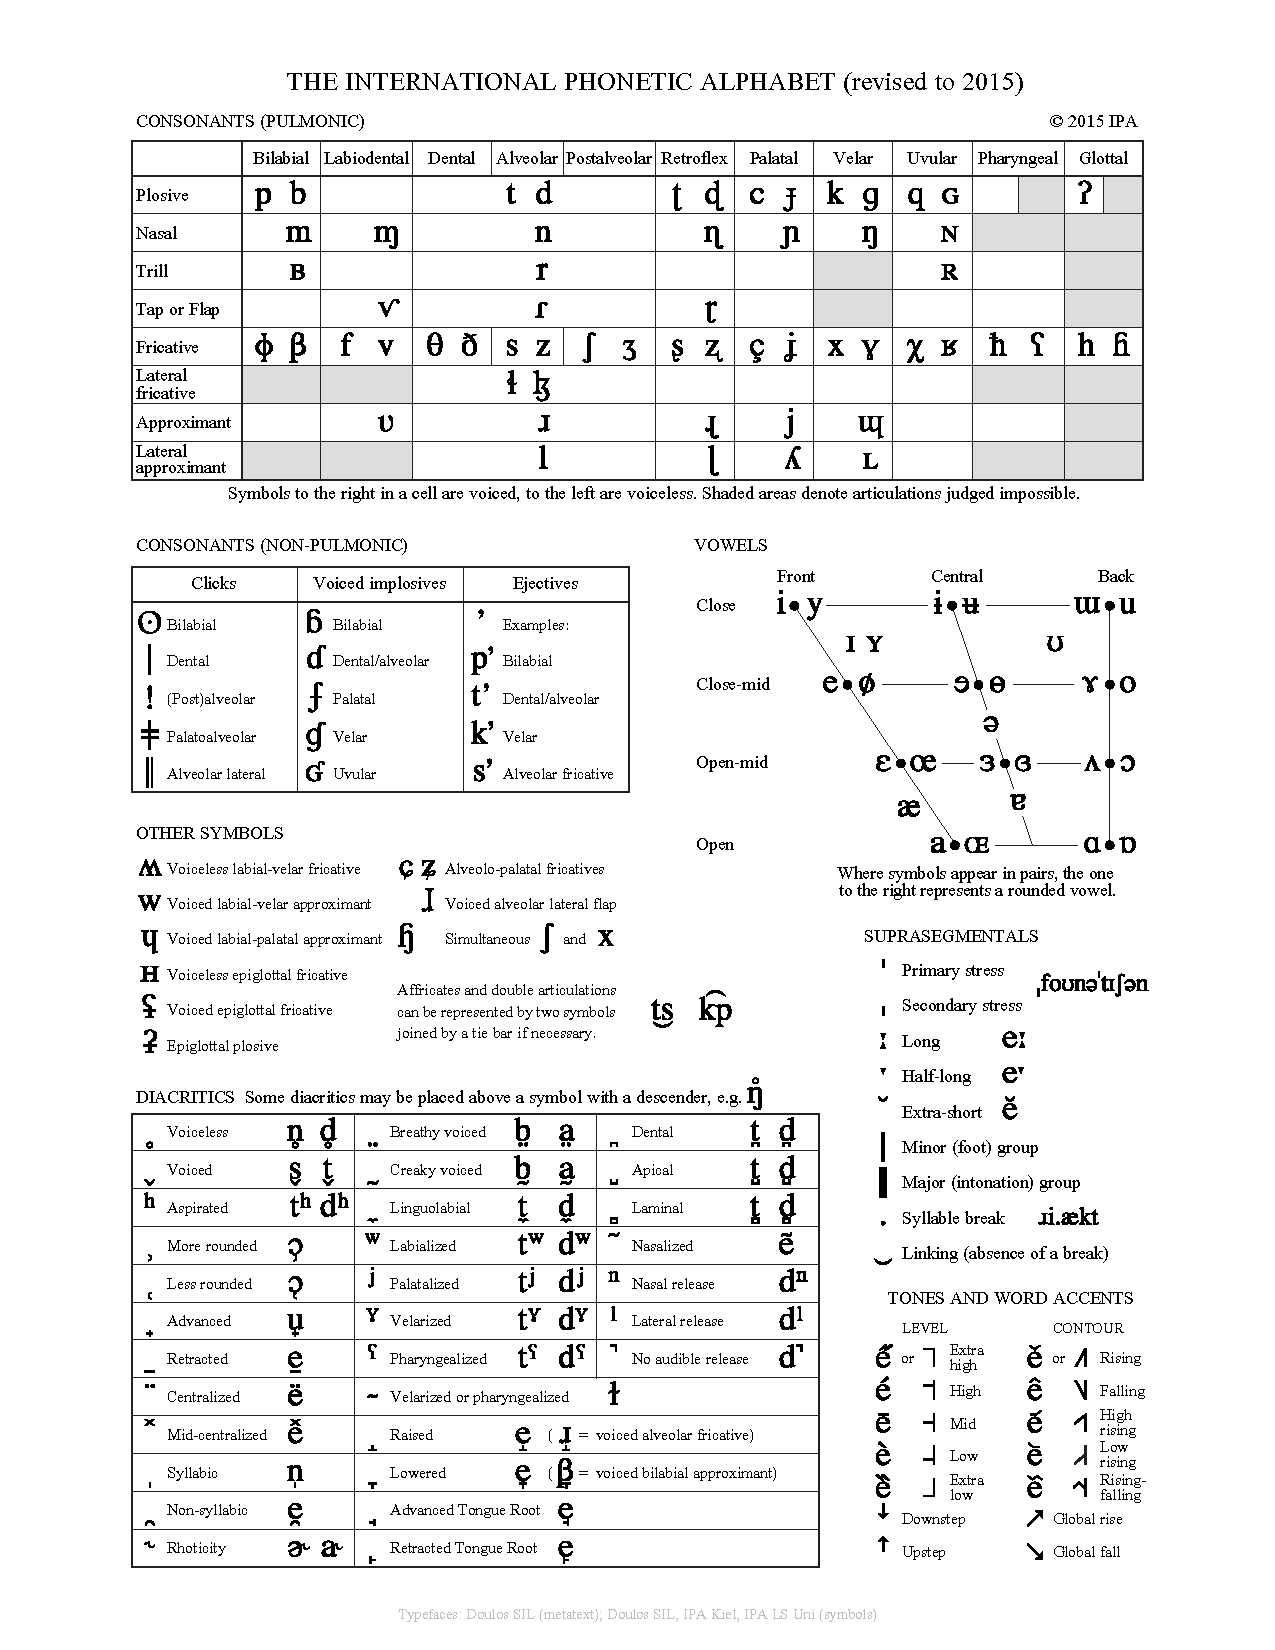
\includegraphics[width=1.3\linewidth]{ipa_chart.pdf}
    \end{center}
    \stepcounter{myfigure}
    \caption[Full IPA chart]{This is the full IPA chart, last updated in 2015}
    \label{fig:ipa_chart}
  \end{figure}



